% Исходный LaTeX-код (c) Пётр Калинин
% Код распространяется по лицензии GNU GPL (!)

\header{Элементарные примеры}
\label{backtrack_elementary}

Я тут долго думал, стоит сначала объяснять общую идею или все-таки сначала 
пример разбирать. Буду сначала пример, так, наверное, понятнее.

\lheader{Перебор всех $2^k$ двоичных чисел из $k$ разрядов}

\note{Это, пожалуй, единственный пример, когда в некоторых случаях имеет смысл писать прямой 
перебор. Действительно, перебрать все $k$"=значные двоичные числа можно легко:
\mbox{\tt for i:=0 to (1 shl k) - 1 do}
"--- и $i$ пробежит все $k$"=значные двоичные числа. Это бывает полезно, например, в 
динамике по подмножествам или динамике по профилю, но нередко бывает полезнее 
рекурсивный перебор, который мы и будем тут разбирать.}

Пусть нам надо, например, вывести на экран все $k$"=значные двоичные числа (их 
всего, очевидно, $2^k$). Напишем следующую программу 

\begin{codesample}\begin{verbatim}
var a:array...

procedure check;
var i:integer;
begin
for i:=1 to k do
    write(a[k]);
writeln;
end;

procedure find(i:integer);
begin
if i>k then begin
   check;
   exit;
end;
a[i]:=0;
find(i+1);
a[i]:=1;
find(i+1);
end;

begin
readln(k);
find(1);
end.
\end{verbatim}
\end{codesample}

и посмотрим, как она работает. Есть массив $a$, в котором будет накапливаться 
наше двоичное число, по одной цифре в элементе массива.

Процедура $check$ делает то, что надо сделать с очередным найденным числом: 
выводит его на экран. Если бы надо было делать что-то ещё, она бы делала что-то 
ещё; более подробно я напишу ниже.

Основная часть программы "--- процедура $find$. Её <<\textit{основная идея}>> "--- пусть у нас 
в массиве $a$ первые $i-1$ элементов уже заполнены некоторыми двоичными цифрами, 
т.е. сформировано некоторое начала $k$-битового числа. Тогда результатом вызова 
$find(i)$ будет перебор всех возможных $2^{k-i+1}$ <<концов>> числа, т.е. вызов процедуры $check$ для всех $2^{k-i+1}$ двоичных чисел с заданным началом. (У нас заполнены 
первые $i-1$ элементов, т.е. осталось заполнить $k-i+1$, потому и $2^{k-i+1}$ 
вариантов; $i$ обозначает номер первой незаполненной позиции "--- позиции, откуда надо начинать заполнять массив $a$.)

\lheadernd{Почему это работает?}\label{whyworks}
Попробуем понять, как она работает (т.е. почему сказанное выше про неё верно). 
Можно понять это с нескольких сторон :)

Посмотрим с конца.

Во"-{}первых, как работает $find(k+1)$. Видно, что она просто запускает $check$ и 
выходит. Но именно это она и должна сделать в соответствии с <<основной идеей>>. 
Действительно, вызов $find(k+1)$ обозначает, что первые $(k+1)-1$ элементов массива 
уже заполнены, т.е. заполнены \textit{все} $k$ элементов, т.е. уже сформировано очередное решение "--- осталось только вывести его на экран.

Рассмотрим теперь работу $find(k)$. Она сделает следующее: поставит в $a[k]$ цифру 
$0$ и вызовет $find(k+1)$, которая (как мы только что видели) выведет массив на 
экран. Потом она поставит в $a[k]$ цифру $1$ и опять вызовет $find(k+1)$, которая 
опять просто выведет решение на экран.

Это полностью соответствует <<основной идее>>. Действительно, первые $k-1$ 
элементов массива уже должны быть заполнены, поэтому осталось только перебрать 
два варианта заполнения последней цифры и вывести оба на экран. Именно это она 
и делает.

Посмотрим теперь $find(k-1)$. К её вызову первые $k-2$ элемента массива уже должны 
быть заполнены, поэтому осталось перебрать все варианты заполнения оставшихся 
двух элементов. Что сделает $find(k-1)$. Она поставит в $a[k-1]$ ноль и вызовет 
$find(k)$, которая, как мы видели, переберёт все возможные $1$"=циферные окончания и 
выведет их на экран. Далее, когда $find(k)$ отработает, произойдёт возврат в 
$find(k-1)$, она поставит в $a[k-1]$ единицу и опять запустит $find(k)$, которая 
переберёт все возможные $1$"=циферные окончания такого начала. Видно, что таким 
образом $find(k-1)$ переберёт все возможные $2$"=циферные окончания решения, 
сформированного перед её вызовом, т.е. отработает в соответствии с <<основной 
идеей>>.

Теперь $find(k-2)$. Ей надо перебрать все возможные $3$"=циферные окончания. Она 
поставит ноль в $a[k-2]$ и вызовет $find(k-1)$, которая, как мы только что видели, 
действительно перебирает все $2$"=циферные окончания. После этого поставит единицу 
в $a[k-2]$ и опять вызовет $find(k-1)$. Поскольку все $3$"=циферные окончания "--- это либо 
ноль и $2$"=циферное окончание, либо единица и $2$"=циферное окончание, то вызов 
$find(k-2)$ действительно перебирает все $3$"=циферные окончания.

И так далее [на самом деле выше я просто тремя несколько различными способами
описывал фактически одно и то же. Работа $find(k-2)$ ничем принципиально не 
отличается от $find(k-1)$ и т.п.].

Вообще, $find(i)$ надо перебрать все окончания от $i$"=ой цифры до конца массива. Но все 
такие окончания "--- это либо ноль и окончание от $i+1$-ой до конца, либо единица 
и окончание от $i+1$-ой до конца. В соответствии с этим $find(i)$ и ставит в $a[i]$ 
ноль и вызывает $find(i+1)$, тем самым перебирая все окончания от $i+1$-ой цифры до 
конца, потом ставит в $a[i]$ единицу и опять вызывает $find(i+1)$.

Теперь ясно, что $find(1)$ перебирает все $k$"=значные окончания пустого числа (т.е. 
числа, в котором ноль цифр), т.е. действительно решает задачу.

\begin{wrapfigure}{l}{6.5cm}
{\newcommand{\0}{\hbox to 1.5cm{\hfill 0\hfill}}
\newcommand{\1}{\hbox to 1.5cm{\hfill 1\hfill}}
\rule{6cm}{0.5pt}\\
 $
\displaystyle
\left|
\frac{\displaystyle
\0
  \left|
  \frac{\displaystyle
  \0
    \left|
    \frac{\displaystyle
    \0
    }{\displaystyle
    \1
    }
    \right.
  }{\displaystyle
  \1
    \left|
    \frac{\displaystyle
    \0
    }{\displaystyle
    \1
    }
    \right.
  }
  \right.
}{\displaystyle
\1
  \left|
  \frac{\displaystyle
  \0
    \left|
    \frac{\displaystyle
    \0
    }{\displaystyle
    \1
    }
    \right.
  }{\displaystyle
  \1
    \left|
    \frac{\displaystyle
    \0
    }{\displaystyle
    \1
    }
    \right.
  }
  \right.
}
\right.
\cdots
 $\\
\rule{6cm}{0.5pt}
}
\end{wrapfigure}


Посмотрим теперь на ту же работу с начала (в смысле, не с конца) [на самом деле 
то, что я тут пишу "--- это в некотором смысле тавтология. Я одно и тоже 
переписываю в разных вариантах, надеясь, что хотя бы одним вы проникнетесь :)]. 


Все двоичные числа можно представить в виде таблицы, приведённой слева:
в первую очередь разделяем числа по первой цифре, во вторую очередь по второй и 
т.д. В соответствии с этим и работают процедуры $find$. Можно себе представить 
ось времени направленную вертикально вниз, с верхней границей таблицы "--- моментом 
запуска $find(1)$, нижней границей "--- концом запуска $find(1)$. Самая левая 
вертикальная черта отражает работу $find(1)$: она работает все время. Следующая 
вертикальная черта состоит из двух частей: они отражают работу $find(2)$. 
Процедура $find(2)$ будет запущена дважды ($find(1)$ запустит её дважды), потому 
две черты. Каждый запуск $find(2)$ запустит $find(3)$ два раза "--- итого четыре 
запуска $find(3)$, отражаемые четырьмя кусочками третьей вертикальной прямой. 
(все четыре копии будут работать одна за другой, а не одновременно, ведь 
вертикальная ось "--- это ось времени). Видно, что делает каждая процедура $find$: 
она ставит в соответствующую ячейку массива $a$ ноль, потом один (цифры справа от 
вертикальной черты, соответствующей запуску процедуры), и для каждой цифры 
запускать процедуру $find$ <<следующего уровня>> (две вертикальные черты ещё 
правее). Видно и как будет в итоге меняться массив $a$: вначале в нем все нули, 
потом, начиная с правых цифр, в нем меняются нули на единицы и т.д., в конце 
"--- все единицы.

Наконец, ещё один вариант представления того, что происходит. Он, может, не так 
ясно разъясняет работу, но весьма полезен для понимания идей перебора вообще.

\lheader{Дерево решений}
Все множество решений (в нашем случае решения "--- это все $k$"=битовые двоичные 
числа) можно представить в виде дерева, делая сначала разделение решений по 
первому биту, потом по второму и т.д.:

\begin{wrapfigure}{l}{8cm}%
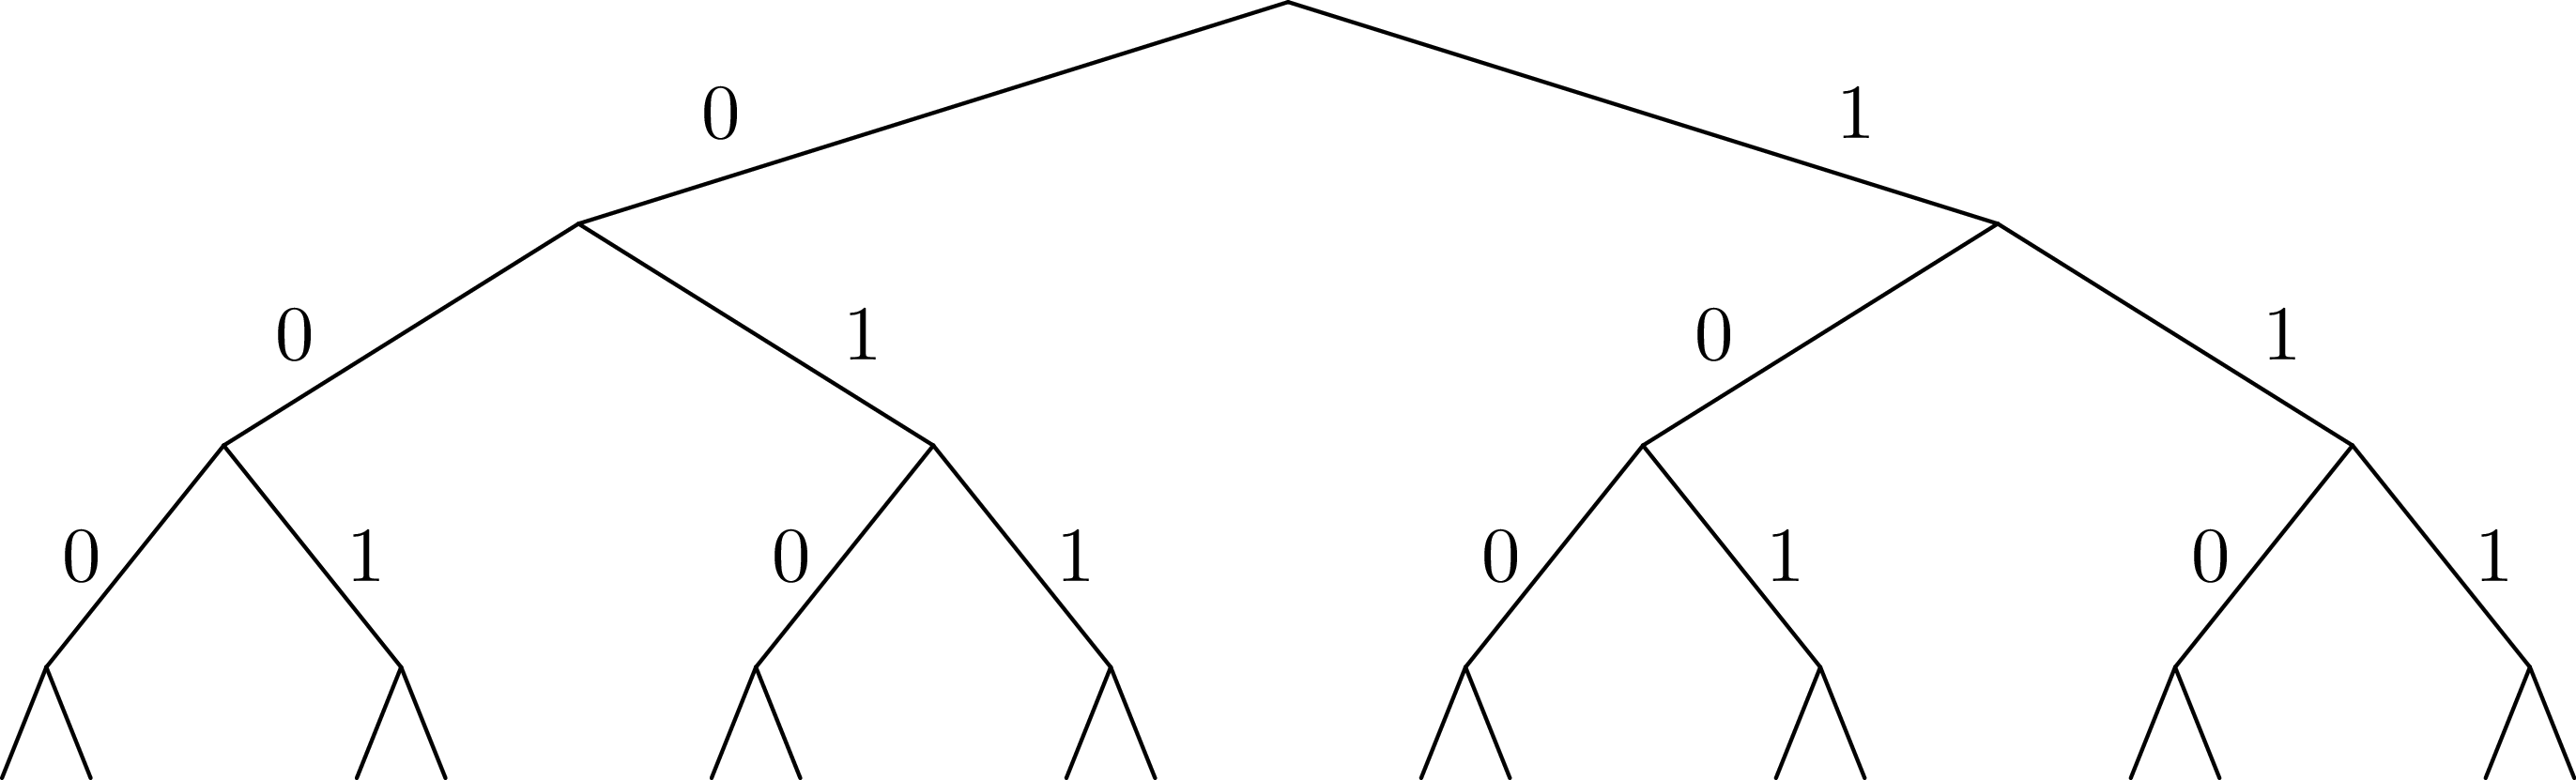
\includegraphics[width=8cm]{texts/01_1_elementary/tree.1}%
\end{wrapfigure}

С этой точки зрения работа процедуры $find$ очень похожа на поиск в глубину по этому 
дереву (на самом деле, она и есть поиск в глубину). Мы сначала обходим левое 
поддерево корня, проходя ребро и рекурсивно запускаясь от левого сына корня, 
после окончания обхода обходим правое поддерево, проходя соответствующее ребро 
и рекурсивно запускаясь от правого сына. Представление о дереве решений нам 
будет очень полезно в дальнейшем.

Я надеюсь, что в этом месте вполне понятно, как работает процедура $find$.

\lheader{О процедуре $check$}
Обратите внимание, что на самом деле, как видно, нам совсем не важно, что делает процедура $check$. Эта процедура делает то, что нужно в данной конкретной задаче сделать с 
найденным решением (в нашем случае "--- с найденным $k$-битным числом): надо его 
вывести на экран "--- выведем, надо в файл сохранить "--- сохраним, надо проверку 
какую-нибудь сделать "--- сделаем и т.д. Для написания  собственно \textit{перебора} не важно, что она будет делать; основная задача перебора "--- поставлять процедуре $check$ одно за другим решения. Но именно процедура $check$ будет делать то, зачем мы делали 
перебор: считать такие объекты, или проверять, подходит ли объект под условие, или 
искать объект минимальной стоимости\dots


\lheader{Общая идеология поиска}
Итак, нам надо перебрать объекты из некоторого множества. Более конкретно "---
вызвать процедуру $check$ для каждого объекта. Таким образом, 
основная задача перебора будет состоять в том, чтобы вызвать процедуру $check$ 
для всех объектов из нашего множества.

Обычно объекты из множества можно задавать некоторым массивом, элементы 
которого принимают те или иные значения. В приведённом выше примере это был 
массив $a$ "--- массив двоичных цифр; везде ниже я аналогичные массивы тоже буду 
обозначать $a$. Обычно перебрать все подходящие значения очередного элемента 
массива $a$ легко; в приведённом выше примере каждый элемент массива $a$ мог 
принимать два значения: ноль и один.

Тогда перебрать все объекты можно с помощью следующей процедуры:

\begin{codesampleo}\begin{verbatim}
procedure find(i:integer);
begin
if (выбраны все элементы, т.е. сформировано некоторое решение) then begin
   check;
   exit;
end;
Для каждого возможного значения a[i] begin
    a[i]:=это значение;
    find(i+1);
end;
end;
\end{verbatim}
\end{codesampleo}

Комментарии:
\begin{enumerate}
\item Проверка на то, что решение сформировано. В простейшем случае это будет 
просто if~$i>k$, как выше, но могут быть и более сложные варианты (например, если 
число элементов не фиксировано).
\item Цикл по возможным значениям $a[i]$. Опять"=таки, в каждом конкретном случае, 
конечно, свой. Как правило, это будет цикл $for$, нередко с вложенным $if$, например,
\begin{codesampleo}\begin{verbatim}
for j:=1 to n do if (j может быть значением a[i]) then begin
    a[i]:=j;
    find(i+1);
end;
\end{verbatim}
\end{codesampleo}
примеры будут ниже.
\end{enumerate}

Эта процедура $find$ работает аналогично приведённому выше примеру (и вообще, все 
процедуры $find$ в переборе работают аналогично друг другу): считая, что начало 
из $i-1$ элемента фиксировано, перебирает все возможные окончания. Она смотрит, 
какой может быть $i$-й элемент, перебирает все его значения, и для каждого 
запускает рекурсивно $find(i+1)$, которая переберёт все окончания, считая первые 
$i$ элементов фиксированными.

Процедура $check$ делает то, что надо сделать с решением. В большинстве случаев 
это проверка, удовлетворяет ли найденное решение каким-либо требованиям 
(примеры см. ниже), поэтом так и названа. Как я уже много раз говорил, 
конкретный вид процедуры $check$ нам не важен.

\lheader{Перебор всех $k$-значных чисел в $n$-ичной системе счисления}
(Всего таких чисел $n^k$)\nopagebreak

(Зачем я все время привожу, сколько таких объектов: просто для того, чтобы вы 
могли лишний раз проверить, что вы понимаете, о каких объектах идёт речь: посчитайте сами в уме количество таких объектов и сравните; никакой больше нагрузки это не несёт.)

\begin{codesampleo}\begin{verbatim}
procedure find(i:integer);
var j:integer;
begin
if i>k then begin
   check;
   exit;
end;
for j:=0 to n-1 do begin
    a[i]:=j;
    find(i+1);
end;
end;
\end{verbatim}
\end{codesampleo}

Я надеюсь, что работа этой процедуры если и не очевидна после всего 
вышеизложенного, то за несколько секунд становится понятной. Единственное 
отличие от примера 1 "--- то, что надо перебирать не $2$ цифры, а $n$, и потому 
перебор делаем циклом.

\lheader{Разложение числа $N$ в степени двойки}
Несколько притянутый за уши пример: по данному числу $N$ определить, можно ли его 
представить в виде суммы $k$ степеней двойки, не обязательно различных.

\note{Конечно, эту задачу, как и многие другие, которые мы тут будем обсуждать, вполне можно решать другими, более разумными, быстрыми и правильными методами, чем перебором, но мы тут будем обсуждать именно переборные решения в качестве иллюстрации общих концепций.}

Будем перебирать все возможные наборы из $k$ степеней двойки; соответственно, в 
массив $a$ будем записывать последовательно эти степени.

\begin{codesample}\begin{verbatim}
procedure check;
var j:integer;  
    s:longint;
begin
s:=0;
for j:=1 to k do
    s:=s+a[j];
if s=n then begin
   for j:=1 to k do
       write(a[j],' ');
   writeln;
end;
end;
procedure find(i:integer);
var j:integer;
begin
if i>k then begin
   check;
   exit;
end;
for j:=0 to 30 do begin
    a[i]:=1 shl j;
    find(i+1);
end;
end;
\end{verbatim}
\end{codesample}

Во-первых, я ещё раз привожу текст процедуры $check$, чтобы вы видели, что она 
будет делать здесь (а она проверяет, подходит ли нам такое решение, и, если да, 
то выводит его на экран).

Во-вторых, обратите внимание на перебор всех степеней двойки циклом по $j$. 
Можно, конечно, этот перебор написать и по-другому, например так:

\begin{codesampleo}\begin{verbatim}
a[i]:=1;
while a[i]<1 shl 30 do begin
      find(i+1);
      a[i]:=a[i] shl 1;
end;
\end{verbatim}
\end{codesampleo}
или типа того: не суть важно, как написать перебор, главное, правильно написать, не 
забыв ни одного варианта; в частности, обратите внимание, что этот вариант кода по сравнению с приведённым в 
процедуре $find$ выше перебирает на одну степень двойки меньше. (\taskn{Контрольный вопрос}|Видите, почему?||Посмотрите, как будет заканчиваться цикл while.||На последней итерации цикла \texttt{a[i]} станет \texttt{1 shl 29}, оно обработается, потом удваивается, становится равным \texttt{1 shl 30}, и происходит окончание цикла. Значение \texttt{1 shl 30} не обрабатывается.|)

Я надеюсь, что в остальном идея работы процедуры понятна.

\task|Напишите эту программу (собственно, я надеюсь, что и предыдущие 
   программы вы написали). 
  Потестите её (обратите внимание, что тут время работы от $n$ не зависит, 
   только от $k$, потому имеет смысл брать и большие $n$). Найдите в ней баг и 
   придумайте, как его исправить. 
 Кроме того, заметьте, что одно и то же решение выводится несколько 
   раз, отличаясь перестановкой слагаемых. Придумайте, как это исправить (может 
   быть, вам поможет сначала почитать следующий пример, но лучше подумайте 
   сначала, не читая примера дальше).
||Для поиска бага попробуйте включить ключи компилятора.||Баг в том, что при вычислении суммы чисел в $check$ может быть переполнение. Можно, например 
 написать
\begin{codesampleo}\begin{verbatim}
procedure check;
var j:integer;  
    s:longint;
begin
s:=0;
for j:=1 to k do if s<=n-a[j]  then
    s:=s+a[j]
else exit;
if s=n then begin
   for j:=1 to k do
       write(a[j],' ');
   writeln;
end;
end;
\end{verbatim}
\end{codesampleo}
Должно бы вроде работать.

Исключить повторный вывод одного и того же решения можно, потребовав, чтобы слагаемые неубывали.
\begin{codesampleo}\begin{verbatim}
for j:=0 to 30 do if 1 shl j>=a[i-1] begin
\end{verbatim}
\end{codesampleo}
|



\lheader{Перебор всех сочетаний из n по k (т.е. всех $C_n^k$)} Хочется также в массив $a$ 
записывать выбранные элементы. Но тут возникнут две  
проблемы: во"=первых, надо, чтобы все элементы были различными, во"=вторых, чтобы 
сочетания не повторялись из-за изменения порядка элементов (ведь $\{1,3\}$ и $\{3,1\}$ 
"--- это одно и то же сочетание).

\task|Можно, конечно, это проверять в процедуре $check$. Т.е. процедура $find$ 
будет фактически работать по предыдущему примеру, а процедура $check$ будет отбирать то, 
что нужно. Напишите такую программу. Обратите внимание на то, чтобы не 
брать одно и то же сочетание несколько раз.||||Проверить неповторяемость можно, проверяя, что 
элементы в массиве идут в неубывающем порядке "--- т.е. идея та же, что и ниже в основном тексте|

Обе проблемы решаются одной идеей: будем требовать, чтобы в массиве $a$ элементы 
шли строго по возрастанию. Тогда получаем следующую процедуру $find$ (считаем, что 
элементы, из которых мы собираем сочетание, занумерованы от $0$ до $n-1$): 

\begin{codesampleo}\begin{verbatim}
procedure find(i:integer);
var j:integer;
begin
if i>k then begin
   check;
   exit;
end;
for j:=0 to n-1 do if j>a[i-1] then begin
    a[i]:=j;
    find(i+1);
end;
end;
\end{verbatim}
\end{codesampleo}


Обратите внимание на нетривиальный $for$. Проверка гарантирует, что все элементы 
будут идти по возрастанию. На самом деле, очевидно, что весь $for$ можно заменить на 

\begin{codesampleo}\begin{verbatim}
for j:=a[i-1]+1 to n-1 do
\end{verbatim}
\end{codesampleo}
без всяких $if$; так и надо писать, пример выше приведён скорее для того, чтобы 
вы поняли, как иногда бывает надо проверять дополнительные условия.

Кроме того, заметьте, что теперь не все ветви перебора заканчиваются 
формированием решения. Действительно, если, например, $k=3$, а мы на первом же 
уровне перебора (т.е. в $find(1)$) возьмём $a[1]=n-1$, то видно, что на втором уровне 
(т.е. в $find(2)$) нам будет нечего делать. Аналогично, если $k=3$, а на первом 
уровне берём $a[1]=n-2$, то на втором придётся взять $a[2]=n-1$ и на третьем делать 
нечего.

\task|а) Напишите эту программу. Обратите внимание на подготовку вызова
   $find(1)$; проверьте, что перебираются действительно \textbf{все} сочетания (например, 
   выводя их в файл и проверяя при маленьких $n$ и $k$). \par
 б) Добавьте в программу код, который выводит (на экран или в файл) <<лог>> работы 
   рекурсии (например, выводя при присвоении $a[i]:=j;$ на экран строку `\texttt{a[i]=j}',
   сдвинутую на $i$ пробелов от левого края строки: вам этот вывод покажет, чт\'{о} на
   самом деле делает программа и пояснит предыдущий абзац); этот <<лог>> лучше
   выводить вперемешку с найденными решениями, чтобы видеть, какая ветка рекурсии
   чем закончилась. Подумайте над тем, как  исправить то, что описано в предыдущем
   абзаце, т.е. как сделать так, чтобы каждая ветка рекурсии заканчивалась нахождением решения.
||а) Включите ключи компилятора; б) Подумайте, почему некоторые ветки не находят решения и как это 
исправить.
||а) $find(1)$ обращается к $a[0]$. Чтобы все работало, надо перед вызовом $find(1)$ установить 
$a[0]=-1$ или ещё меньше :), иначе сочетания не смогут начинаться с нуля и т.п.
(Именно потому я и предложил считать, что элементы у нас занумерованы от $0$ до $n-1$, а не от $1$ 
до $n$: в последнем случае достаточно было поставить $a[0]=0$ и это было бы легче не заметить :) ). 
\par
б) Понятно, что в $find(i)$ бессмысленно ставить $a[i]=n-1$, если только $i$ не равно $k$. Вообще, ясно, 
что не имеет смысла ставить $a[i]>n-(k-i)-1$ (вроде так, может быть $\pm1$, подумайте), т.к. 
элементов на оставшиеся места не хватит. Поэтому стоит делать цикл от $a[i-1]+1$ до $n-(k-i)-1$.|

Замечу ещё, что в этой задаче можно написать процедуру $find$ немного по"=другому. 
А именно, будем ей теперь передавать два параметра, $i$ и $x$. Смысл параметра $i$ 
тот же, что и раньше, а $x$ обозначает, начиная с какого числа надо перебирать 
очередной элемент:

\begin{codesampleo}\begin{verbatim}
procedure find(i:integer;x:integer);
var j:integer;
begin
if i>k then begin
   check;
   exit;
end;
for j:=x to n-1 do
    a[i]:=j;
    find(i+1,j+1);
end;
end;
\end{verbatim}
\end{codesampleo}

На самом деле тут $x$ будет всегда равен $a[i-1]+1$, просто, может быть, такую 
процедуру проще понять.

Смысл процедуры $find$ теперь такой: перебрать все возможные окончания нашего 
сочетания, в которых все элементы не меньше, чем $x$.

Вообще, иногда и в других задачах имеет смысл передавать процедуре $find$ 
дополнительные параметры, которые так или иначе ограничивают область перебора 
очередного элемента, точнее, подсказывают, какие значения элемента стоит 
перебирать. Как правило, их (параметры) всегда можно выразить через уже 
сформированную часть решения, но иногда проще их передавать, чем каждый раз пересчитывать.

\lheader{Перебор всех $n!$ перестановок из $n$ чисел (от $1$ до $n$)}

Здесь из проблем, перечисленных в начале предыдущего примера, осталась одна: 
надо, чтобы все элементы перестановки были различными. Порядок же, наоборот, 
как раз таки важен, и поэтому такой приём, как в прошлом примере, здесь не 
пойдёт. 

Поэтому применим другой приём, который весьма полезен бывает во многих задачах 
на перебор. А именно, введём второй глобальный массив, массив $was$, в котором 
будем фиксировать, использовали ли мы каждое число. Т.е. очередным элементом в 
перестановку будем ставить только те числа, которые ещё не были использованы.
(Естественно, в массиве $a$ будем хранить получающуюся перестановку).

\begin{codesampleo}\begin{verbatim}
var was:array...

procedure find(i:integer);
var j:integer;
begin
if i>n then begin
   check;
   exit;
end;
for j:=1 to n do if was[j]=0 then begin
    a[i]:=j;
    was[j]:=1;
    find(i+1);
    was[j]:=0;
end;
end;
\end{verbatim}
\end{codesampleo}

Во"=первых, тут у нас количество элементов в объекте, которое раньше было $k$, 
теперь равно $n$ "--- общему количеству элементов, поэтому такое условие выхода из 
рекурсии.

Во-вторых, как собственно работает процедура $find(i)$. Она перебирает, какой 
элемент надо поставить на $i$-е место. Этот элемент не должен быть использован 
ранее (т.е. не должен уже стоять в массиве $a$), потому и проверка \texttt{if was[j]=0}.
Далее, она ставит этот элемент в массив $a$, помечает, что он теперь 
использован и запускает $find(i+1)$ для перебора всех <<хвостов>> текущей 
перестановки. При этом переборе элемент $j$ использован уже не будет, т.к. в 
$was[j]$ помечено, что он уже взят. Надеюсь, что работа процедуры понятна.

\taskn{\deftaskname{} (элементарное)}|Напишите программу перебора всех $A_n^k$ "--- всех 
размещений из $n$ по $k$ (в них, в отличии от $C_n^k$, порядок важен).|
||
|То же, что и для перестановок, только проверка на выход из рекурсии будет \texttt{if i>k}, а не 
\texttt{if i>n}.|


А теперь обратите особое внимание на строчку
\begin{codesampleo}\begin{verbatim}
    was[j]:=0;
\end{verbatim}
\end{codesampleo}
в приведённом выше тексте. Обсуждению её мы посвятим почти всё оставшееся в
текущей части время. Она является примером очень важной идеи, пожалуй, самого важного
правила, которое есть при написании переборных программ. Именно несоблюдение
этого правила (а точнее, забывание про него), на мой взгляд, является одним из
основных источников ошибок в переборе, поэтому \textsc{всегда, когда пишете перебор,
помните про него}:

\textsc{Процедура $find$ должна всегда возвращать назад все изменения, которые она 
производит} (за небольшими исключениями, когда вы \textsc{чётко осознаете}, почему 
некоторое изменение можно не возвращать назад), причём лучше всего возвращать 
назад изменения сразу после вызова $find(i+1)$.


Здесь процедура $find$ пометила, что элемент $j$ использован. Строка 
\begin{codesampleo}\begin{verbatim}
    was[j]:=0;
\end{verbatim}
\end{codesampleo}
отыгрывает назад это изменение, что вполне логично, т.к. процедура $find(i+1)$ 
переберёт все окончания, у которых на $i$-м месте стоит $j$, и после этого мы будем 
перебирать другие варианты, в которых элемент $j$ больше (пока) не используется.
Очевидно, что, если бы этой строки не было, это привело бы к 
глобальным ошибкам в работе программы. Если вам это не очевидно, то тщательно продумайте этот 
момент; это важно и на самом деле это показывает, насколько хорошо вы понимаете работу перебора. 
Если никак не можете понять, в чем дело, вспомните аргументацию раздела \ref{whyworks}, 
и промоделируйте аналогично работу в этом случае.

Другие программы могут делать изменения в других (глобальных) переменных; 
примеры будут потом. И всегда надо тщательно проверить, что откат назад 
происходит. В простых случаях поможет просто вручную изменять значения назад, 
как в примере выше. В более сложных случаях может быть не так просто отыграть 
все изменения. В таком случае может помочь сохранение старых переменных в стеке 
процедуры и восстановление их целиком, например

\begin{codesampleo}\begin{verbatim}
type tWas=array...
var was:tWas;

procedure find(i:integer);
var j:integer;
    oWas:tWas;  {old was}
begin
if i>n then begin
   check;
   exit;
end;
oWas:=was; {сохраняем старый массив}
for j:=1 to n do if was[j]=0 then begin
    a[i]:=j;
    was[j]:=1;
    find(i+1);
    was:=oWas; {восстанавливаем его}
end;
end;
\end{verbatim}
\end{codesampleo}

Один из минусов этого подхода "--- то, что довольно активно расходуется память в 
стеке, но зато не надо тщательно следить за всеми изменениями, которые делает 
$find$, и не надо думать, какой же командой надо откатить изменения (здесь это было очевидно, но могут быть более сложные случаи).

Обратите внимание вот ещё на что: кажется, что эту же процедуру можно написать 
по-другому, так, чтобы она восстанавливала массив $was$ \textit{до} работы:

\begin{codesampleo}\begin{verbatim}
procedure find(i:integer);
var j:integer;
    oWas:tWas; {old was}
begin
if i>n then begin
   check;
   exit;
end;
oWas:=was; {сохраняем старый массив}
for j:=1 to n do begin
    was:=oWas; {восстанавливаем}
    if was[j]=0 then begin
       a[i]:=j;
       was[j]:=1;
       find(i+1);
    end;
end;
end;
\end{verbatim}
\end{codesampleo}

Но не очевидно, что этот вариант будет работать, т.к. последнее изменение не 
будет <<откачено>>, и после окончания процедуры $find$ массив was будет не таким, 
каким он был раньше (на самом деле его тут же исправит восстановление массива 
на уровень выше, но как минимум не очевидно, что это будет работать, надо думать). 
Поэтому старайтесь восстанавливать все изменения как можно раньше.

Кстати, ещё обратите внимание: \textit{все} программы, которые мы до сих пор писали, изменяют массив 
$a$ и \textit{не} откатывают изменения. Поймите, почему \textit{это} не страшно.

И, наконец, последнее замечание в этой части. В Borland Pascal есть своеобразный 
баг при отладке рекурсивных процедур. А именно, как известно, в BP есть 
следующие четыре основных клавиши, управляющие работой программ при отладке:
\begin{itemize}
\item F9: выполнять программу до конца или до ближайшего breakpoint,
\item F8: выполнить текущую строку,
\item F7: если в текущей строке нет вызовов функций и процедур, кроме стандартных, то 
    выполнить текущую строку (то же, что и F8),
    иначе войти в отладку вызова функции, присутствующего в данной строке.
\item F4: Run to cursor: выполнять программу, пока она не дойдёт до выполнения 
    строки, на которой стоит курсор.
\end{itemize}
    
Так вот, в BP клавиша F8 действует на самом деле примерно как F4 по следующей 
строке: она не выполняет текущую строку \textit{полностью}, а выполняет программу до тех 
пор, пока впервые не станет выполняться следующая строка кода. Если в программе 
нет рекурсивных вызовов, эти два варианта равносильны, а вот если рекурсия есть, 
то все хуже. Пример: наша любимая процедура $find$
\begin{codesampleo}\begin{verbatim}
procedure find(i:integer);
begin
...
  ...
  find(i+1);
  ...
end;
\end{verbatim}
\end{codesampleo}
Если на строке $find(i+1);$ вы нажмёте F8, то программа остановится не тогда, 
когда эта $find(i+1)$ отработает полностью, а когда \textit{какой-нибудь} вызов $find$ с 
этой же строки отработает. Как правило, это будет глубоко в рекурсии. Например, 
вы нажали F8 на этой строке при $i=1$ "--- программа остановится на следующей строке, но не 
при $i=1$, а (скорее всего) типа при $i=k$ и т.п. (т.е. когда она \textit{впервые} дойдёт до 
строки, следующей за $find(i+1);$). Это может оказаться очень  
неожиданно, т.к. у вас сразу меняются значения $i$ и всех остальных переменных, 
причём нет так, как вы ожидали, но, если помнить об этой особенности, то ничего 
неожиданного нет. Но в таком случае отладка рекурсивных программ становится 
весьма нетривиальной. Чтобы сделать <<настоящее>> F8, т.е. отработать этот вызов 
полностью, приходится на следующей строке ставить breakpoint с условием 
$i=<\mbox{тому, что надо}>$, и жать F9.

Ещё раз замечу, что это относится не только к перебору, но к любым рекурсивным 
процедурам.

В Delphi (и FP?) этого бага вроде нет.

\lheader{Совсем общая концепция перебора}
Все задачи до сих пор у нас в основном крутились вокруг некоторого массива $a$, который мы последовательно заполняли. 
Действительно, очень многие задачи, решаемые рекурсивным перебором, можно представить именно так
"--- как задачу перебора возможных заполнений некоторого массива $a$.

Но перебор, на самом деле, намного более мощная идея. 
Пусть у нас есть задача, в которой нам надо перебрать набор решений, а каждое решение образуется
некоторой последовательностью <<элементарных>> шагов. 
То есть пусть мы можем говорить о каких"=то <<состояниях>>, <<позициях>> в этой задаче, из каждого
состояния/позиции есть набор <<ходов>> в другие позиции, и нам надо найти последовательность ходов,
приводящую к требуемой <<конечной>> позиции (или посчитать, сколько таких последовательностей есть,
или найти оптимальную из них и т.д.) 
При этом будем считать, что у нас нет зацикливаний: мы не можем из одной позиции сделать несколько ходов
и вернуться в нее же. 

Тогда эта задача несложно решается перебором. 
Процедура \verb`find` будет работать так: она будет считать, что у нас уже сформирована некоторая позиция. 
Процедура будет перебирать все возможные ходы из этой позиции, и рекурсивно запускать себя из полученных позиций. 

Простейший пример "--- карточный пасьянс типа косынки. 
У нас есть текущая позиция (не будем сейчас обсуждать, как ее представить в программе; будем также считать,
что мы знаем все закрытые карты, иначе ответ не определен).
Мы хотим определить, сойдется ли пасьянс, т.е. есть ли такая последовательность наших действий, при которой пасьянс сходится.

Если бы в каждый момент у нас был бы лишь один возможный ход, то задача была бы простой: мы просто делали бы эти ходы
и посмотрели бы на результат.

Но в <<косынке>> из каждой позиции у нас может быть несколько ходов. 
Поэтому процедура \verb`find` будет работать так: по данной позиции она будет перебирать все возможные ходы
и рекурсивно запускаться для поиска дальнейшего решения.

\begin{codesampleo}\begin{verbatim}
procedure find; 
begin
if ходов нет then
    check; // процедура проверит, сошелся ли пасьянс
    exit;
end;
for все возможные ходы do begin
    сделать ход
    find
    откатить ход назад (!)
end;
end;
\end{verbatim}
\end{codesampleo}

Еще пример "--- крестики"=нолики на поле $3\times 3$. 
Пусть нам надо написать программу, которая будет искать оптимальный в некотором смысле ход из данной позиции.
Для простоты оптимальность определим так: оптимальным будем называть такой ход, после которого мы точно сможем выиграть
независимо от ходов противника. 
Если таких ходов несколько, выберем любой из них. 
Если таких ходов нет, но есть ходы, гарантирующие нам ничью, то выберем любой из ничейных ходов.
Если же все ходы ведут к нашему проигрышу (при условии идеального соперника), то сообщим об этом.

(Отмечу, что <<оптимальность>> хода можно было бы определить и сложнее, например, попытаться как"=то учесть возможность
противнику ошибиться. Но мы так усложнять не будем.)

Для этого просто переберем все возможные способы развития партии, начиная с некоторой позиции. 
Теперь у нас будет не процедура \verb`find`, а функция.
Она будет принимать в качестве параметра, кто (крестики или нолики) ходят сейчас и будет возвращать,
кто выигрывает при идеальной игре обоих соперников. Код будет примерно такой:
\begin{codesampleo}\begin{verbatim}
function find(player:integer):integer; // player=-1 -- нолики, player=1 --- крестики
begin
проверить, не окончена ли игра (т.е. выиграл ли уже кто-то и не заполнено ли поле)
if игра окончена then begin
   if крестики выиграли then result:=1
   else if нолики выиграли then result:=-1
   else result:=0; // ничья
   exit;
end;
// переменная optimal хранит номер выигрывающего игрока (-1, 0 или 1)
// изначально худший для нас вариант --- выигрывает противник
optimal:=-player; // -player как раз дает противника
for i:=1 to 3 do
    for j:=1 to 3 do if клетка (i,j) свободна then begin
        сходим в клетку (i,j)
        winner:=find(-player); // рекурсивно переберем дальнейшие варианты 
                               // и узнаем, кто выигрывает
        if player=1 then
            if winner>optimal then // для крестиков мы хотим 
                optimal:=winner;  // номер выигрывающего игрока как можно больше
                  // т.е. крестики лучше ничьей, а ничья лучше ноликов
        else // player=-1 --- нолики
            if winner<optimal then // для ноликов мы хотим 
                optimal:=winner;  // номер выигрывающего игрока как можно меньше
                  // т.е. нолики лучше ничьей, а ничья лучше крестиков
        
        отменим ход в (i,j) // откатимся!!
    end;
// теперь optimal --- выигрывающий игрок при самом лучшем нашем ходе
result:=optimal; 
end;
\end{verbatim}
\end{codesampleo}

\task|(Сложное) Напишите эту программу полностью и доведите ее до такого состояния, чтобы можно было играть с компьютером
в крестики"=нолики.
|||||

Так можно решать практически любую игру, в которой не бывает зацикливаний. 
(А на самом деле если зацикливания возможны, то первый вопрос "--- а что происходит в реальной игре в таким случае? 
Ведь вряд ли игра на самом деле будет продолжаться до бесконечности?
В шахматах, например, при трехкратном повторении позиции объявляется ничья, поэтому зацикливания невозможны,
просто надо хранить все позиции, которые уже встречались.)

Правда, конечно, есть проблема "--- если игра сложная, с множеством ходов и длинными партиями, то времени перебрать
все возможные партии не хватит. Например, в шахматах таким перебором решаются разве что малофигурные эндшпили.

Еще пример такой задачи:

\task|(Задача 159 c \verb`informatics.mccme.ru`) Радиолюбитель Петя решил собрать детекторный приемник. 
Для этого ему понадобился конденсатор емкостью $C$ мкФ. 
В распоряжении Пети есть набор из $n$ конденсаторов, емкости которых равны $c_1$, $c_2$, \dots, $c_n$, соответственно. 
Петя помнит, как вычисляется емкость параллельного соединения двух конденсаторов ($C_{new} = C_1 + C_2$) 
и последовательного соединения двух конденсаторов ($C_{new} = C1\cdot C2/(C1+C2)$). 
Петя хочет спаять некоторую последовательно-параллельную схему из имеющегося набора конденсаторов, такую, 
что ее емкость ближе всего к искомой (то есть абсолютная величина разности значений минимальна). 
Разумеется, Петя не обязан использовать для изготовления схемы все конденсаторы.

Напомним определение последовательно-параллельной схемы. Схема, составленная из одного конденсатора, – последовательно-параллельная схема. 
Любая схема, полученная последовательным соединением двух последовательно-параллельных схем, – последовательно-параллельная, 
а также любая схема, полученная параллельным соединением двух последовательно-параллельных схем, – последовательно-параллельная. 
Обратите внимание, что это определение не допускает произвольные схемы, 
а только полученные именно последовательностью параллельных или последовательных соединений.||||TODO|

\lheader{Задачи к части \ref{backtrack_elementary}}
Я надеюсь, что вы решите одну-две задачи и хотя бы \textit{серьёзно} (хотя бы день) 
подумаете над остальными (или решите их), прежде чем переходить к части \ref{backtrack_cuts}.
Часть из (нормальных переборных) решений этих задачи использует идеи, про которые я буду 
рассказывать в части \ref{backtrack_cuts}, но будет неплохо, если вы додумаетесь до них сами :) хотя бы в этих 
задачах (а я буду стараться рассказывать для общего случая), или если напишете что-то хоть и 
корявое, но работающее.

До того, как переходить к части \ref{backtrack_cuts}, порешайте эти задачи. Точнее, сначала убедитесь, что 
материал части \ref{backtrack_elementary} у вас <<осел>> в голове, и что вы часть \ref{backtrack_elementary} понимаете (а для этого прорешайте 
задачи из текста части \ref{backtrack_elementary}), потом решайте задачи. Если не решите (подумав над задачами хотя бы 
некоторое время, день-два), смотрите подсказки. Попробуйте учесть их и подумать 
над задачами ещё. Потом разберите решения. Может быть, последние три задачи вам 
покажутся нетривиальными "--- ну хотя бы попробуйте их решать\dots

\task|Напишите программу перебора всех последовательностей из 0 и 1 без $k$ 
нулей подряд, в которых всего $n$ символов. (Например, при $k=2$ и $n=3$ это будут 
последовательности 010, 011, 101, 110 и 111). Основной задачей программы будет посчитать, 
сколько таких последовательностей всего, но имеет смысл выводить их на экран (или в 
файл) для проверки.\par
а) Напишите эту программу, модифицировав пример 1, т.е перебирая \textsc{все} 
последовательности из 0 и 1 длины $n$, и проверяя, что последовательность 
<<правильная>>, только в процедуре $check$.\par
б) Напишите программу, которая будет перебирать \textsc{только} такие 
последовательности, т.е. чтобы \textsc{каждая} ветка перебора заканчивалась 
нахождением решения, и в процедуре $check$ проверки не были бы нужны.\par
в) (дополнительный пункт, не имеющий отношения к перебору) Если вы раньше не сталкивались с такой задачей, то
попробуйте найти закономерность ответов при фиксированном $k$ (т.е. сначала
посмотрите на ответы на задачу при $k=2$ и найдите в них закономерность, потом
поищите закономерность при $k=3$, потом при $k=4$ и т.д.) Кстати, не забудьте, что 
тестить имеет смысл и очевидный случай $k=1$ :)
||б) Можно дописывать ноль, только если текущая последовательность заканчивается меньше, чем на $k-1$ нулей. Можно каждый раз считать заново, на сколько нулей заканчивается текущая последовательность, а можно передавать в $find$ дополнительный параметр "--- 
сколько нулей стоят в конце текущей последовательности. Попробуйте 
написать оба способа.
||б) Ну понятно: будем ставить ноль только при условии, что среди предыдущих $k-1$ символов есть единицы.
Для $k=2$ это написать просто:
\begin{codesampleo}\begin{verbatim}
procedure find(i:integer);
begin
if....
end;
a[i]:=1;
find(i+1);
if a[i-1]=1 then begin {ставим ноль, только если предыдущий символ --- 1}
   a[i]:=0;
   find(i+1);
end;
end;
\end{verbatim}
\end{codesampleo}
только тут надо будет убедиться, что $a[0]=1$, чтобы последовательности могли \textit{начинаться} с нуля.

Для б\'{о}льших $k$ можно писать цикл, который будет считать, на сколько нулей заканчивается текущая последовательность (только аккуратно с $a[0]$, $a[-1]$ и т.д., чтобы 
последовательности могли начинаться с нулей) "--- попробуйте это написать!, "--- а можно это не считать каждый раз заново, а передавать в $find$ дополнительным параметром:
\begin{codesampleo}\begin{verbatim}
procedure find(i,l:integer);
begin
if...
end;
a[i]:=1;
find(i,0);  {на конце текущей последовательности единица, т.е. ноль нулей :) }
if l<k-1 then begin  {можно дописать еще один ноль}
   a[i]:=0;
   find(i+1,l+1);  {стало на один ноль больше}
end;
end;
\end{verbatim}
\end{codesampleo}
в главной программе тогда надо вызывать $find(1,0)$ и никаких проблем с $a[0]$ и т.п.

в) Закономерность обсудим в теме "Динамическое программирование".
|

\task|Паросочетание в произвольном графе. Рассмотрим граф с $2N$ (т.е. чётным) 
количеством вершин. Паросочетанием в нем назовём набор из $N$ рёбер, у которых все 
концы различны (т.е. каждая вершина соединена ровно с одной другой: разбиение 
вершин на пары). [В олимпиадном программировании обычно рассматривается только 
паросочетание в \textsc{двудольном} графе, т.к. там есть простой эффективный алгоритм. 
Но у нас граф будет произвольным и мы будем решать задачу перебором]. 
[Т.е. смысл этой задачи на самом деле "--- чтобы вы умели перебирать все 
разбиения на пары]\par
а) Напишите программу, которая будет перебирать все разбиения вершин на пары и 
проверять, является ли такое разбиение паросочетанием (т.е. все ли нужные ребра 
присутствуют в нашем графе).\par
б) Считая, что граф полный и взвешенный, напишите программу, которая найдёт 
паросочетание наименьшего веса.
||На самом деле вариант а) отличается от варианта б) только процедурой $check$ и 
возможными отсечениями (см. раздел II). Основное в процедуре $find$ у них одно и то же: перебор 
всех разбиений $N$ объектов на пары. Пожалуй, основной нетривиальностью, над которой придётся подумать, тут будет то, что
в $find(i)$ может оказаться, что $i$"=я вершина уже с кем-нибудь спарена. Можно 
предложить два варианта решения проблемы:\par
1. Можно в массиве хранить \textit{список выбранных рёбер} (!): он тогда будет 
\begin{codesampleo}\begin{verbatim}
array of record a,b:integer; end;
\end{verbatim}
\end{codesampleo}
переменная $i$ в $find$ будет указывать, какое ребро мы хотим выбрать (в смысле, $i=1$ 
значит, что мы ещё не выбрали ни одного ребра, $i=2$ "--- что выбрали одно и 
т.д.). 

В процедуре $find$ теперь ищем первую вершину, которая ещё не <<спарена>>, т.е. не 
является концом ни одного из взятых ещё рёбер, её обязательно берём, и 
перебираем ей пару. Для того, чтобы не тратить время на проверку, <<спарена>> ли 
вершина, можно завести массив $was$, в котором отмечать, спарены ли вершины (и не 
забывать откатывать!)

Это решение довольно прямо идёт по естественной идеологии перебора: нам надо выбрать $N$ рёбер "--- так и будем их последовательно выбирать, записывая номера выбранных в массив $a$.
\par
2. Но можно делать и, как мне кажется, проще. Можно в массиве $a$ хранить номер <<парной>> вершины к данной вершине: т.е. $a[i]$ "--- 
номер вершины, парной к $i$, или ноль, 
если вершина пока ещё не спарена. В частности, для уже спаренных вершин обязательно должно быть $a[a[i]]=i$. Процедура $find(i)$ будет перебирать пары к 
$i$-ой вершине. А именно, если она уже с кем-то спарена, то перебирать нечего, 
иначе перебираем все свободные вершины в качестве пары. Массив $was$ тут не 
нужен, т.к. <<спаренность>> вершины можно проверять, проверяя $a[i]=0$. Обратите 
\textsc{особое внимание} на то, что здесь придётся откатывать \textsc{изменения в массиве} $a$! "--- это довольно редкий случай, но вот вам пример, когда это действительно нужно.
||Общий текст для пунктов а) и б) (как уже было отмечено в подсказках, процедура $find$ почти не отличается для них); в части II вам будет предложено придумать отсечения 
здесь.

В соответствии с вариантом 1 из подсказок:
\begin{codesampleo}\begin{verbatim}
var a:array... of record a,b:integer; end;
    was:array...
    
procedure find(i:integer); {выбираем i-е ребро паросочетания}
var j,k:integer;
begin
if i>n then begin
   check; {процедура check разная в вариантах а и б}
   exit;
end;
{найдем первую свободную вершину}
for j:=1 to 2*n do {в графе 2*n вершин!}
    if was[j]=0 then break;
{теперь j --- номер первой свободной (не входящей в паросочетание) вершины.
Добавим ее в паросочетание и будем искать парную к ней}
was[j]:=1;
for k:=1 to 2*n do {можно k:=j+1 to 2*n, т.к. до j-ой все точно спарены}
    if was[k]=0 then begin {тут хочется проверить наличие ребра, но пока мы считаем, что это делаем в check}
       was[k]:=1;
       a[i].a:=j;
       a[i].b:=k;
       find(i+1);
       was[k]:=0;
    end;
was[j]:=0;
{обратите внимание, что именно здесь!
или надо was[j]:=0 внутри цикла, но и was[j]:=1 тоже!}
end;
\end{verbatim}
\end{codesampleo}

В соответствии с вариантом 2 из подсказок:
\begin{codesampleo}\begin{verbatim}
var a:array... of integer;

procedure find(i:integer); {выбираем парную к i-й вершине}
var j:integer;
begin
if i>2*n then begin {количество вершин в графе --- 2*n, а не n!}
   check;
   exit;
end;
if a[i]<>0 then {парная вершина уже выбрана, перебирать нечего}
   find(i+1)
else {надо перебрать все варианты}
     for j:=i+1 to 2*n do if a[j]=0 then begin {i+1 --- т.к. все до i-ой уже точно спарены}
         {спарим i-ую и j-ую вершины}
         a[i]:=j;
         a[j]:=i;
         find(i+1);
         a[i]:=0;
         a[j]:=0;{!!!обязательно, т.к. иначе i-я и j-я будут считаться еще спаренными!}
     end;
end;
\end{verbatim}
\end{codesampleo}
|\label{matching}

\task|Напишите программу перебора всех разложений числа $N$ 
 на натуральные слагаемые.\par
 Вариант 1: ровно на $k$ слагаемых\par
   а) считая, что слагаемые могут повторяться и что порядок слагаемых важен (т.е. что $2+1$ и $1+2$ "--- это разные решения);\par
   б) считая, что порядок слагаемых не важен, т.е. выводя только одно разложение 
      из разложений $2+1$ и $1+2$, при этом допуская одинаковые слагаемые;\par
   в) считая, что все слагаемые должны быть различны, при этом порядок слагаемых 
      не важен.\par
 Вариант 2: на сколько угодно слагаемых в тех же трёх подвариантах (а, б и в)\par
 Написав программы, прежде чем тестировать их, ответьте в уме на такой вопрос: ваша (уже написанная!) программа в варианте а) будет  при $n=3$ выводить решения $1+2$ и $2+1$. А при $n=2$ она будет выводить $1+1$ один раз или два раза (во второй раз как будто переставив единички)?
||Можно ввести дополнительную глобальную переменную, в которой хранить текущую сумму 
слагаемых, в процедуре $find$ увеличивать её на то слагаемое, которое поставили, и не забывать 
потом вернуть назад. Можно поступить по-другому: передавать в процедуру $find$ дополнительный 
параметр, который обозначает, сколько ещё осталось разложить 
(т.е. $N - \mbox{\it (сумма уже выбранных слагаемых)}$). При этом тогда очередное слагаемое будет ограничено сверху значением этого параметра.
Вариант 2: подумайте, какое должно быть условие выхода из рекурсии.
||Варианты а, б, в различаются только тем, что в в) достаточно потребовать, чтобы слагаемые строго возрастали, в б) "--- неубывали, а в а) это все не имеет значения.

Разберём вариант 1в): заведём глобальную переменную $s$, в которой храним текущую сумму. 

\begin{codesampleo}\begin{verbatim}
var s:...

procedure find(i:integer);
var j:integer;
begin
if i>k then....
end;
for j:=a[i-1]+1 to n-s do begin {слагаемое должно быть больше предыдущего, но явно не больше, чем n-s}
    a[i]:=j;
    s:=s+j;
    find(i+1);
    s:=s-j; {откатываем изменения !!!}
end;
end;
\end{verbatim}
\end{codesampleo}

Обратите внимание, что в процедуре $check$ придётся проверять, что $s=n$.

Варианты 1б и 1в отличаются только нижней границей цикла: $a[i-1]$ и $1$ соответственно.

Вариант 2 отличается, в первую очередь, условием выхода из рекурсии. Тут несложно видеть, что 
условие выхода из рекурсии будет \texttt{if s=n}, и в $check$ проверять ничего не придётся.

Можно писать и по-другому, не вводя переменную $s$, а в процедуру $check$ передавая оставшуюся сумму $rem$; теперь процедура $find$ будет иметь смысл <<разложить число $rem$ на слагаемые>> с какими-нибудь условиями. Например для 2а:
\begin{codesampleo}\begin{verbatim}
procedure find(i:integer;rem:integer); 
var j:integer;
begin
if rem=0 then begin {если rem=0, то мы разложили уже всё N, т.е. нашли решение}
   check;
   exit;
end;
for j:=a[i-1]+1 to rem do begin
    a[i]:=j;
    find(i+1,rem-a[i]); {осталось разложить rem-a[i]}
end;
end;
\end{verbatim}
\end{codesampleo}
Можно в $find$ передавать и текущую сумму, и т.д. "--- как вам приятнее.
|

\task|Задача <<Числа>>. Дана последовательность из $N$ чисел. За одно действие разрешается удалить любое число (кроме крайних), заплатив за это штраф, равный произведению этого числа на сумму двух его соседей. Требуется удалить все числа (кроме двух крайних) с минимальным суммарным штрафом. 

У этой задачи есть (не самое тривиальное) динамическое решение, но напишите переборное решение. Тут надо перебрать все варианты удаления чисел и выбирать из них тот, который даст минимальный штраф.
||В массиве $a$ будем хранить последовательность удалений (на самом деле, тут нам массив $a$ практически не будет нужен). Стоит (в добавок к массиву $a$) хранить ещё один
глобальный массив, в котором будет храниться текущее состояние чисел, и ещё глобальную 
переменную "--- текущий штраф. При удаление очередного числа надо откорректировать глобальный массив, удалив из него это число (и сдвинув другие числа), а также изменить текущий штраф. Не забудьте все отыгрывать назад. 

Но более продвинутый вариант "--- хранить текущее состояние чисел связным списком, а не массивом, тогда удалять и добавлять элементы просто.
||Разберём в разделе \ref{Numbers_Adv}.|\label{Numbers_simple}

\task|(Какая-то довольно искусственная задача, но хорошо подходит для иллюстрации одной из идей далее). Посчитать количество последовательностей из $m$ нулей и $n$ единиц, удовлетворяющих следующих условиям. Первое условие: никакие две единицы не должны стоять рядом. Таким образом единицы делят последовательность на несколько групп из подряд идущих нулей. Второе условие: количество нулей в последовательных группах должно неубывать, и при этом в соседних группах должно отличаться не более чем на 1. Эта задача имеет динамическое решение, но напишите перебор.
||Простую программу перебора написать несложно, только лучше перебирать не последовательности из 
нулей и единиц, а сразу способы разбиения $m$ нулей на данное количество групп. Т.е. написать функцию $count(g,m)$, которая 
будет считать число способов разбиения $m$ нулей на $g$ групп с учётом второго условия, а в ответ выводить 
$count(n-1,m)+2\cdot count(n,m)+count(n+1,m)$, поскольку возможны четыре варианта:\par
1. Первый и последний символы искомой последовательности "--- единицы, тогда групп нулей у нас $n-1$ и потому таких последовательностей $count(n-1,m)$.\par
2. Первый символ "--- единица, последний "--- ноль, тогда групп нулей $n$ и таких последовательностей $count(n,m)$.\par
3. Первый символ "--- ноль, последний "--- единица, тогда групп нулей $n$ и таких последовательностей опять-таки $count(n,m)$.\par
4. Первый и последний символы "--- ноли, тогда групп нулей $n+1$ и таких последовательностей $count(n\hm+1,m)$.\par
Функция же $count$ будет инициализировать и запускать перебор нужных разбиений (т.е. и будет той <<главной программой>>, откуда мы запускаем $find(1)$). Массив $a$ будет хранить количество нулей в очередной группе. Можно проверять отличие соседних групп на 1 только в $check$, а можно и по ходу перебора.

Но интереснее постараться сделать так, чтобы (почти) все ветки заканчивались нахождением 
решения. Для этого надо, во-первых, сразу в переборе перебирать только те разбиения, где 
количества нулей в соседних группах или равно, или отличается на единицу, а во-вторых, 
проверять, хватит ли нам нулей на оставшиеся группы; это мы ещё будем обсуждать в разделе \ref{Perestroika_adv}.
||Обсудим в разделе \ref{Perestroika_adv}.|\label{Perestroika_simple}